% ----------------------------------------------------
% DAB Processing
% ----------------------------------------------------
\documentclass[class=report,11pt,crop=false]{standalone}
% Page geometry
\usepackage[a4paper,margin=25mm,top=25mm,bottom=25mm]{geometry}

% Font choice
\usepackage{lmodern}

% Use IEEE bibliography style
\bibliographystyle{IEEEtran}

% Line spacing
\usepackage{setspace}
\setstretch{1.20}

% Ensure UTF8 encoding
\usepackage[utf8]{inputenc}

% Language standard (not too important)
\usepackage[english]{babel}

% Skip a line in between paragraphs
\usepackage{parskip}

% For the creation of dummy text
\usepackage{blindtext}

% Math
\usepackage{amsmath}

% Header & Footer stuff
\usepackage{fancyhdr}
\pagestyle{fancy}
\fancyhead{}
\fancyhead[R]{\nouppercase{\rightmark}}
\fancyfoot{}
\fancyfoot[C]{\thepage}
\renewcommand{\headrulewidth}{0.0pt}
\renewcommand{\footrulewidth}{0.0pt}
\setlength{\headheight}{13.6pt}

% Page geometry
\usepackage[a4paper,top=25mm,bottom=25mm]{geometry}

% Epigraphs
\usepackage{epigraph}
\setlength\epigraphrule{0pt}

% Hyperlinks & References
\usepackage{hyperref}
\hypersetup{
    colorlinks=true,
    linkcolor=blue,
    filecolor=blue,      
    urlcolor=blue,
    citecolor=blue,
}
\urlstyle{same}

% Automatically correct front-side quotes
\usepackage[autostyle=false, style=american]{csquotes}
\MakeOuterQuote{"}

% Graphics
\usepackage{graphicx}
\graphicspath{{Images/}{../Images/}}

% Colour
\usepackage{color}
\usepackage[usenames,dvipsnames]{xcolor}

% SI units
\usepackage{siunitx}

% Microtype goodness
\usepackage{microtype}

% Listings
\usepackage{listings}
\definecolor{backgroundColour}{RGB}{250,250,250}
\definecolor{commentColour}{RGB}{73, 175, 102}
\definecolor{identifierColour}{RGB}{196, 19, 66}
\definecolor{stringColour}{RGB}{252, 156, 30}
\definecolor{keywordColour}{RGB}{50, 38, 224}
\definecolor{lineNumbersColour}{RGB}{127,127,127}
\lstset{ 
  language=Matlab,
  captionpos=b,
  backgroundcolor=\color{backgroundColour},
  basicstyle=\footnotesize,        % the size of the fonts that are used for the code
  breakatwhitespace=false,         % sets if automatic breaks should only happen at whitespace
  breaklines=true,                 % sets automatic line breaking
  postbreak=\mbox{\textcolor{red}{$\hookrightarrow$}\space},
  commentstyle=\color{commentColour},    % comment style
  identifierstyle=\color{identifierColour},
  stringstyle=\color{stringColour},
   keywordstyle=\color{keywordColour},       % keyword style
  %escapeinside={\%*}{*)},          % if you want to add LaTeX within your code
  extendedchars=true,              % lets you use non-ASCII characters; for 8-bits encodings only, does not work with UTF-8
  frame=single,	                   % adds a frame around the code
  keepspaces=true,                 % keeps spaces in text, useful for keeping indentation of code (possibly needs columns=flexible)
  morekeywords={*,...},            % if you want to add more keywords to the set
  numbers=left,                    % where to put the line-numbers; possible values are (none, left, right)
  numbersep=5pt,                   % how far the line-numbers are from the code
  numberstyle=\tiny\color{lineNumbersColour}, % the style that is used for the line-numbers
  rulecolor=\color{black},         % if not set, the frame-color may be changed on line-breaks within not-black text (e.g. comments (green here))
  showspaces=false,                % show spaces everywhere adding particular underscores; it overrides 'showstringspaces'
  showstringspaces=false,          % underline spaces within strings only
  showtabs=false,                  % show tabs within strings adding particular underscores
  stepnumber=1,                    % the step between two line-numbers. If it's 1, each line will be numbered
  tabsize=2,	                   % sets default tabsize to 2 spaces
  %title=\lstname                   % show the filename of files included with \lstinputlisting; also try caption instead of title
}

% Caption stuff
\usepackage{caption}
\usepackage{subcaption}

\makenoidxglossaries

\newacronym{radar}{RADAR}{Radio Detection and Ranging}
\newacronym{dab}{DAB}{Digital Audio Broadcasting}
\newacronym{fm}{FM}{Frequency Modulation}
\newacronym{am}{AM}{Amplitude Modulation}
\newacronym{fdm}{FDM}{Frequency Division Multiplexing}
\newacronym{ofdm}{OFDM}{Orthogonal Frequency Division Multiplexing}
\newacronym{cofdm}{COFDM}{Coded Orthogonal Frequency Division Multiplexing}
\newacronym{dvbt2}{DVB–T2}{Digital Video Broadcasting — Second Generation Terrestrial}
\newacronym{em}{EM}{electromagnetic}
\newacronym{icasa}{ICASA}{Independent Communications Authority of South Africa}
\newacronym{ioo}{IOO}{Illuminators of Opportunity}
\newacronym{pr}{PR}{Passive Radar}
\newacronym{qpsk}{QPSK}{Differential Quadrature Phase-Shift Keying}
\newacronym{dqpsk}{DQPSK}{Differential Quadrature Phase-Shift Keying}
\newacronym{etsi}{ETSI}{European Telecommunications Standards Institute}
\newacronym{psk}{PSK}{Phase Shift Keying}
\newacronym{ask}{ASK}{Amplitude-Shift Keying}
\newacronym{fsk}{FSK}{Frequency-Shift Keying}
\newacronym{iq}{IQ}{In-phase and Quadrature}
\newacronym{prs}{PRS}{Phase Reference Symbol}
\newacronym{dft}{DFT}{Discrete Fourier Transform}
\newacronym{fft}{FFT}{Fast Fourier Transform}
\begin{document}
\ifstandalone
\tableofcontents
\fi
% ----------------------------------------------------
\chapter{Digital Audio Broadcasting: Processing Chain Validation}
\epigraph{For my part, whatever anguish of spirit it may cost, I am willing to know the whole truth, to know the worst, and to provide for it.}%
{\emph{---{Patrick Henry}}}
% ----------------------------------------------------

\section{Overview}
This chapter aims to report on the validation steps that were undertaken when designing the \gls{dab} processing chain. These steps formed an integral part of the design task, by both assisting with the debugging of errors while coding, and further ensuring that the final result achieved the project goals. At the end of the chapter, one should be confident that the created \gls{dab} chain indeed worked correctly.

The structure of the chapter follows logically with how the design process itself unfolded. It starts with a validation method that was fairly non-rigorous, but still useful for early-stage understanding and debugging: that being, graphical validation---simply looking at the features of the outputs at various points in the chain. Thereafter, since most the demodulation and remodulation sub-blocks were designed as inverses of each other, corresponding pairs of functions were tested together with random input data, in the so-called "Inverse Relationship" validation tests. Thirdly, the entire chain was tested by running various datasets through the demodulation-remodulation process \emph{twice}, and comparing the results from the first and second iterations---a correct chain would yield the same results after each. Ultimately, then, the entire chain was tested using provided reference data---real-world \gls{dab} signals and the perfect reconstructions thereof. Descriptions and results of these validation steps follow.

\section{Graphical Validation}
This initial validation step consisted of looking at the output values at various points in the processing chain, and considering them graphically. There were two important caveats to this approach. Firstly, it was not an infallible method of testing, as certain correct graphical features could have arisen even with an incorrect underlying algorithm. Secondly, it could not be done for all sub-blocks---only a handful of the chain's functionality lent itself to such analysis. Nonetheless, it was an important tool in the early stages of the design process. The benefit of doing this validation technique was that problems would manifest close their source: for example, a problem with the demultiplexing of the \gls{ofdm} carriers would be immediately visible in that sub-block's output, and could thus be fixed more rapidly.

\subsection{Methodology}
For at least three points in the chain, one could know \emph{a priori} the correct shape or features of the output data: these points being, after the frame synchronisation step (involving the \texttt{prs\_detect} function), after the demultiplexing of the \gls{ofdm} symbols (involving both the \texttt{symbols\_unpacking} and \texttt{ofdm\_demux} functions), and after the demapping of the \gls{dqpsk} data (involving the \texttt{dqpsk\_demap} functions). The inverses of the latter functions were also considered, but are not covered here, as the verification procedures were almost identical.

Validating these sub-blocks' functionality, then, simply involved looking at their outputs and comparing them to what was expected. Some of these plots were already provided in the previous chapter, and shown to be correct, but a handful more will be provided here for clarity.

\subsection{Frame Synchronisation}
Recall that the frame synchronisation process involved using a Matched Filter to detect the location of a pre-defined \gls{prs} within a given \gls{dab} signal. Since the \gls{prs} is usually fairly distinct from the data-carrying symbols, and because each frame is always preceded by a \gls{ns}, it was easy to recognize the beginning of a frame visually. Thus, by comparing the output index from the \texttt{prs\_detect} function to a plot of the original data, one could quickly see if the algorithm was working correctly. As a reminder, this was not a flawless mode of validation, but it provided good initial insight.

The plot in Figure~\ref{fig:mf_out_good} from the previous chapter has already shown the Matched Filter working on perfect data. Graphically, one can easily see that the \gls{prs} was detected, after the guard interval. It was also via graphical intuition that the problem shown in Figure~\ref{fig:mf_out_prefix-problem} was discovered.

For two further examples, Figure~\ref{fig:validation_mf_rtl} and Figure~\ref{fig:validation_mf_raw}, given here, show the detection process working with real-world data. Importantly, the latter of the two figures displays a situation where the input data was not sampled at \(F_s = 2.048\si{\mega\hertz}\), but rather at \(F_s = 2.5\si{\mega\hertz}\). Thus, inadvertently, this plot additionally demonstrated the correct functioning of the \texttt{iq\_resample} sub-block, since the Matched Filter was designed around the \gls{prs}, which was sampled at \(F_s = 2.048\si{\mega\hertz}\). If the resampling was not working, neither would the \gls{prs} detection process.

\begin{figure}[htbp]
  \centering
  \captionsetup{type=figure}
  \begin{subfigure}[t]{\textwidth}
    \centering
    \captionsetup{type=figure}
    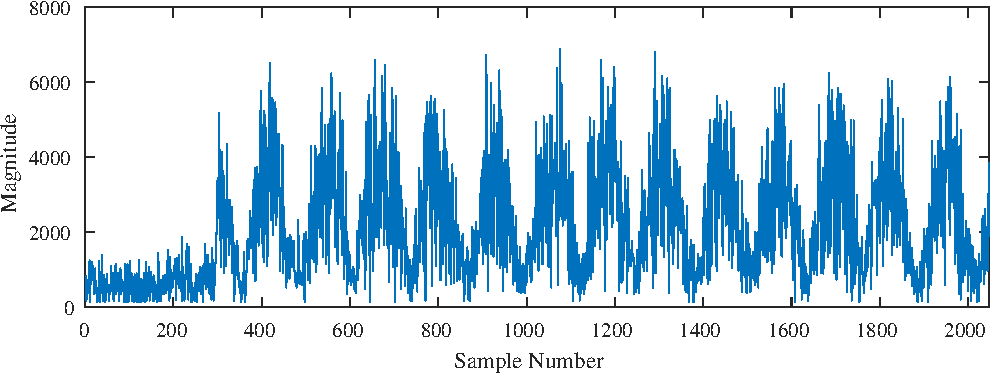
\includegraphics[width=0.6\linewidth]{plots/validation_mf_rtl_signal.pdf}
    \caption{Input to Matched Filter}
    \label{fig:validation_mf_rtl_signal}
  \end{subfigure}%
  \\
  \begin{subfigure}[t]{\textwidth}
    \centering
    \captionsetup{type=figure}
    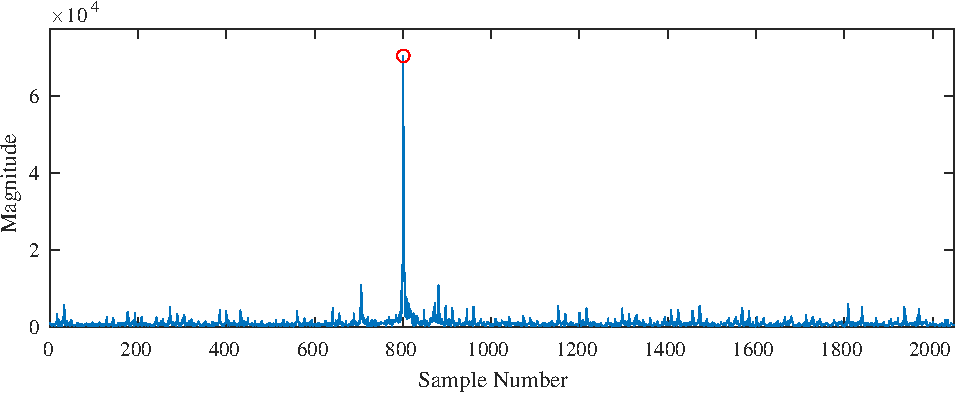
\includegraphics[width=0.6\linewidth]{plots/validation_mf_rtl_peak.pdf}
    \caption{Output from Matched Filter with peak detected}
    \label{fig:validation_mf_rtl_peak}
  \end{subfigure}
  \caption{Plots demonstrating correct functioning of the \texttt{prs\_detect} sub-block using real-world data.}
  \label{fig:validation_mf_rtl}
\end{figure}

\begin{figure}[htbp]
  \centering
  \captionsetup{type=figure}
  \begin{subfigure}[t]{\textwidth}
    \centering
    \captionsetup{type=figure}
    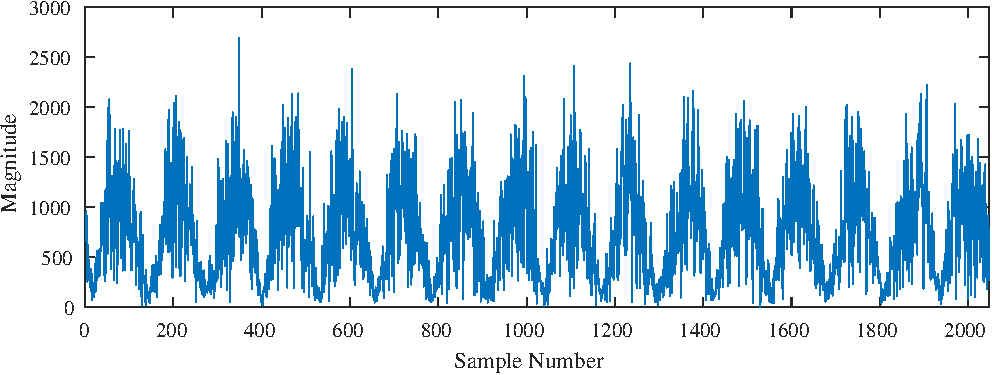
\includegraphics[width=0.6\linewidth]{plots/validation_mf_raw_signal.pdf}
    \caption{Input to Matched Filter}
    \label{fig:validation_mf_raw_signal}
  \end{subfigure}%
  \\
  \begin{subfigure}[t]{\textwidth}
    \centering
    \captionsetup{type=figure}
    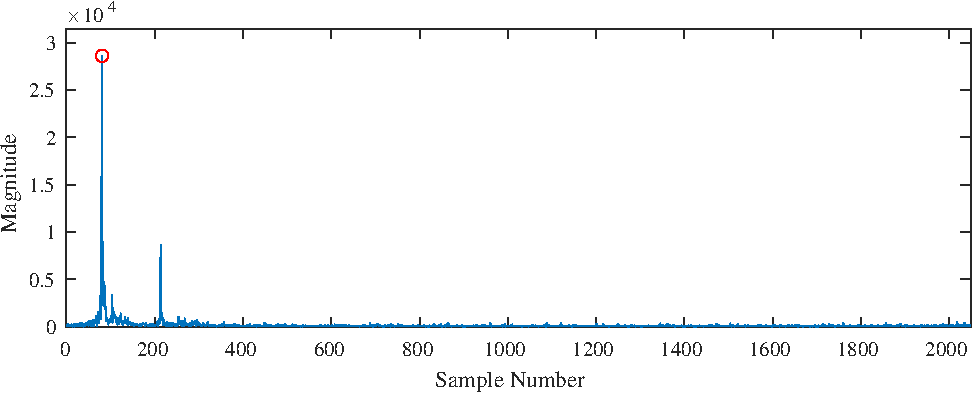
\includegraphics[width=0.6\linewidth]{plots/validation_mf_raw_peak.pdf}
    \caption{Output from Matched Filter with peak detected}
    \label{fig:validation_mf_raw_peak}
  \end{subfigure}
  \caption{More plots demonstrating correct functioning of the \texttt{prs\_detect} sub-block, but using real-world data that was sampled at \(F_s \ne 2.048\si{\mega\hertz}\).}
  \label{fig:validation_mf_raw}
\end{figure}

\subsection{Symbols Unpacking \& OFDM Demultiplexing}
The next two sub-blocks considered were \texttt{symbols\_unpack} and \texttt{ofdm\_demux}. Both were fairly simple blocks, but the validity of the latter's output relied heavily on the validity of the former's correct functionality. Recall that the \gls{ofdm} demultiplexing stage received the \gls{dab} data, after it was split into \(L\) symbols, and the guard intervals were removed. The sub-block then performed a \gls{fft} on the data, thus extracting the \gls{dab} carriers. The plot given in Figure~\ref{fig:ofdm-carriers-perfect}, from the previous chapter, shows an example magnitude plot of these carriers for perfect data, where the spectrum is clearly rectangular and flat in the passband. This implies that the symbols were correctly unpacked.

However, it was worth understanding how such plots would change were the \gls{dab} symbols unpacked \emph{incorrectly}. Suppose the given \gls{dab} frame began at sample \(n_0\), as detected via the \gls{prs}, but the \texttt{symbols\_unpack} function erroneously misaligned the symbols during its unpacking process. The resulting magnitude plots of the \gls{dab} carriers of a single symbol are shown in Figure~\ref{fig:ofdm-carriers-prs} for two situations---one where the symbols have been aligned at \((n_0 - 1)\) samples, the other at \((n_0 + 1)\) samples.

\begin{figure}[htbp]
    \centering
    \captionsetup{type=figure}
    \begin{subfigure}[t]{0.45\textwidth}
      \centering
      \captionsetup{type=figure}
      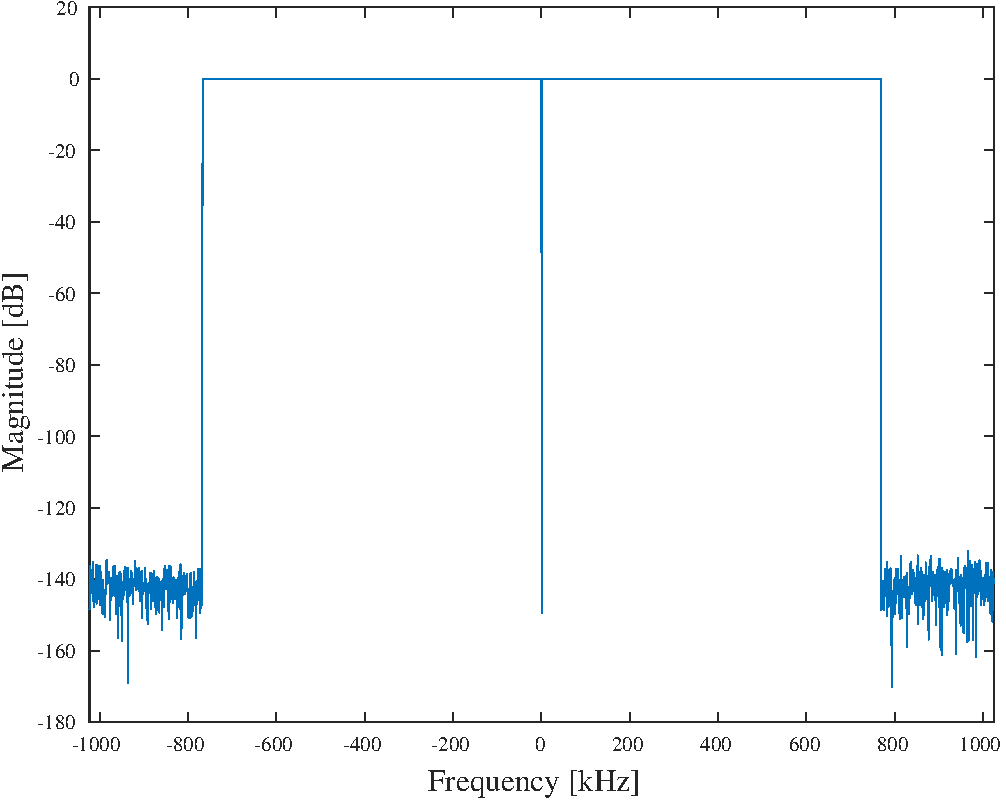
\includegraphics[width=\linewidth]{plots/ofdm-carriers-prs-1.pdf}
      \caption{Symbol aligned at \((n_0 - 1)\) samples}
      \label{fig:ofdm-carriers-prs-1}
    \end{subfigure}%
    ~ 
    \begin{subfigure}[t]{0.45\textwidth}
      \centering
      \captionsetup{type=figure}
      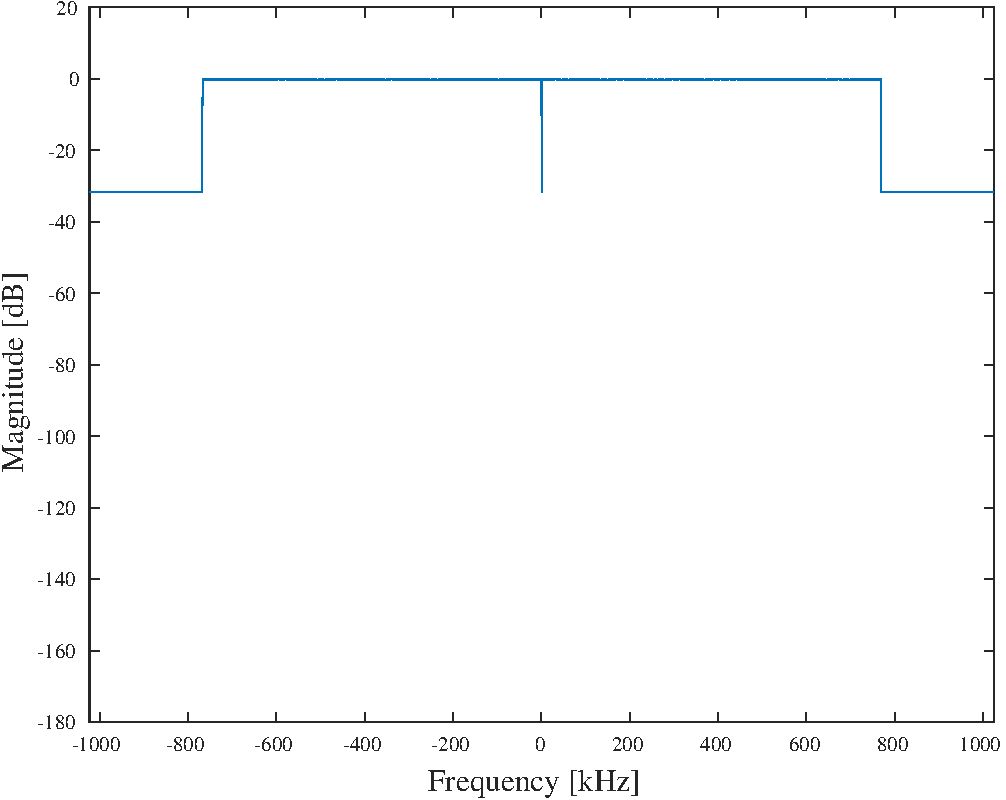
\includegraphics[width=\linewidth]{plots/ofdm-carriers-prs+1.pdf}
      \caption{Symbol aligned at \((n_0 + 1)\) samples}
      \label{fig:ofdm-carriers-prs+1}
    \end{subfigure}
    \caption{Plots showing the magnitude of the \gls{ofdm} carriers for a misaligned \gls{dab} symbol}
    \label{fig:ofdm-carriers-prs}
  \end{figure}

Notice how aligning the symbol prematurely at \((n_0 - 1)\), as shown in Figure~\ref{fig:ofdm-carriers-prs-1}, produced an identical output to that shown before, in Figure~\ref{fig:ofdm-carriers-perfect}, where the passband was flat and the out-of-band noise-floor was virtually zero. However, when the symbol was aligned incorrectly at \((n_0 + 1)\), as shown in Figure~\ref{fig:ofdm-carriers-prs+1}, the noise-floor increased by over \(100\si{\deci\bel}\). As the symbol became more misaligned in the "forward" direction, the resulting \gls{ofdm} carriers became increasingly imperfect. On the other hand, there was leeway for the symbol to be aligned prematurely, without any effect on the resulting functionality.

This effect was due to the guard interval. Remember that a guard interval \emph{precedes} each \gls{dab} symbol. Thus, quite simply, reading a symbol prematurely involved reading the original symbol and some of its guard interval. Reading the symbol too late, however, involved reading the original symbol, as well as the guard interval of the following symbol---which contained completely different data.

It is important to note that these effects were easily visualised when using perfect data, but not so much when using real-world data. The real-world \gls{ofdm} carriers indeed looked somewhat rectangular in magnitude, as seen in Figure~\ref{fig:ofdm-carriers-raw}, but the impact of symbol misalignment was far less pronounced. It is thus recommended that these sub-blocks be designed and initially tested using perfect data.
  
\subsection{DQPSK Demapping}
The demapping of the \gls{dqpsk} data was already discussed somewhat extensively in the previous chapter, and Figures~\ref{fig:dqpsk_demap_perfect},~\ref{fig:dqpsk_demap_rtl} and~\ref{fig:dqpsk_demap_raw} all demonstrated the success of \gls{dqpsk} demodulation, which was able to split the data in four groups of angles, albeit spread out at times. Once again, though, it was worth considering the impact of symbol misalignment on the \texttt{dqpsk\_demap} functionality---using perfect data for clarity. Building on the same two situations from the previous step, Figure~\ref{fig:dqpsk-demap-prs} demonstrates the impact that misalignment had on the \gls{dqpsk} values.

\begin{figure}[htbp]
  \centering
  \captionsetup{type=figure}
  \begin{subfigure}[t]{0.45\textwidth}
    \centering
    \captionsetup{type=figure}
    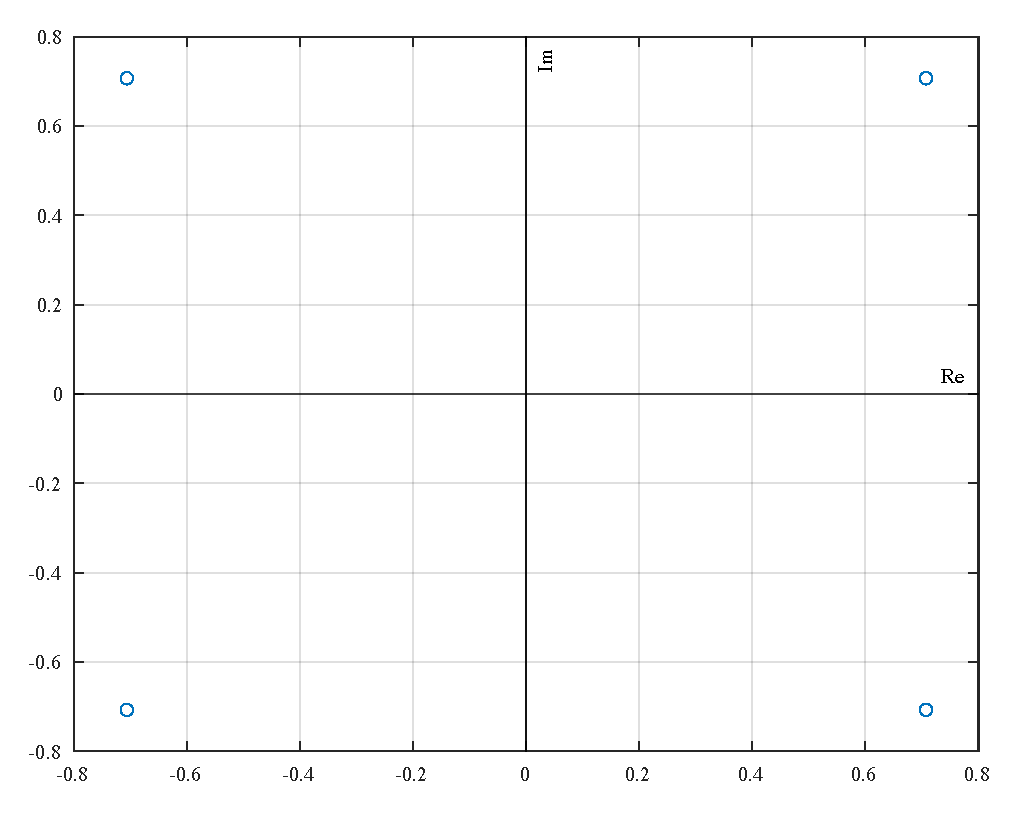
\includegraphics[width=\linewidth]{plots/dqpsk-demap-prs-1.pdf}
    \caption{Symbol aligned at \((n_0 - 1)\) samples}
    \label{fig:dqpsk-demap-prs-1}
  \end{subfigure}%
  ~ 
  \begin{subfigure}[t]{0.45\textwidth}
    \centering
    \captionsetup{type=figure}
    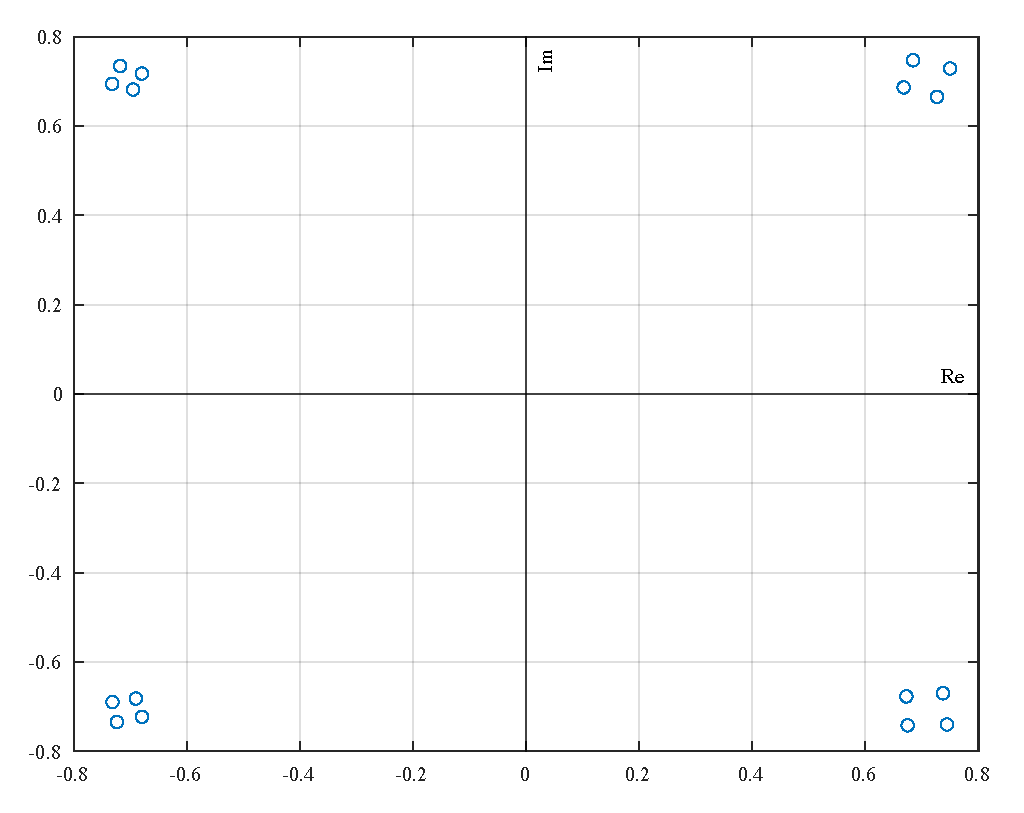
\includegraphics[width=\linewidth]{plots/dqpsk-demap-prs+1.pdf}
    \caption{Symbol aligned at \((n_0 + 1)\) samples}
    \label{fig:dqpsk-demap-prs+1}
  \end{subfigure}
  \caption{Plots showing the values from the \gls{dqpsk} demapping of a misaligned \gls{dab} symbol.}
  \label{fig:dqpsk-demap-prs}
\end{figure}

As was expected, aligning the symbol prematurely, as in Figure~\ref{fig:dqpsk-demap-prs-1}, had no impact on the extracted \gls{dqpsk} data; whereas, aligning the symbol belatedly, as in Figure~\ref{fig:dqpsk-demap-prs+1}, spread out the resulting angles. This was, of course, the same effect of the guard interval as before.

% \subsection{Summary}
% In understanding the effect of symbol misalignment, insight was gained into correct symbol alignment. Thus, by considering the plots at the outputs of each of these sub-blocks, it was 

\section{Inverse Relationship Validation}
An important part of the design rationale for the \gls{dab} processing chain was the idea of "inverse relationships." Essentially, for as many parts of the pipeline as possible, the sub-blocks were designed to have an inverse counterpart. For example, the \texttt{symbols\_pack} function had an inverse in the \texttt{symbols\_unpack} function. Zooming out, the \texttt{demodulation} and \texttt{remodulation} blocks were also somewhat inverted, with one taking a recorded \gls{dab} signal and producing \gls{dab} data, and the other doing the opposite. In fact, this demodulation-remodulation process was the essence of the entire project, with the additional intention that real-world data could be put in on one end, and a perfect reconstruction of this data would be returned. These inverse relationships provided a logical flow to the processing chain, but also provided a good way to test functionality.

\subsection{Methodology}
The essence of this validation process is shown in Figure~\ref{fig:inverse-overview}, where \(f\) and \(f^{-1}\) are two sub-blocks that are being tested together.

\begin{figure}[htbp]
  \centering
  \captionsetup{type=figure}
  \def\svgwidth{0.8\linewidth}
  {\setstretch{0.7} % Line spacing
      \input{../Images/inverse-overview.pdf_tex}}
  \caption{Depiction of the inverse relationship validation process for a generic pair of blocks.}
  \label{fig:inverse-overview}
\end{figure}

The sub-blocks would be considered valid inverses if there was no net change on the input data; thus, an error value was defined:
\begin{equation}
  \mathbf{E} = \mathbf{\tilde{X}} - \mathbf{X}  
\end{equation}
Since this relationship should hold for any input \(\mathbf{X}\), sets of pseudorandom data were provided, and even then, the data was to remain the same at the output. For a valid inverse relationship, then, the maximum value of \(\mathbf{E}\) had to be zero (or extremely close to zero, accounting for numerical inaccuracies) for multiple iterations of arbitrary complex-data as \(\mathbf{X}\).

There are two important notes to make here. Firstly, as was the case for graphical validation, this method was not unerring. Showing that two given sub-blocks demonstrated the above relationship proved that their functionality was inverted, but it said nothing about the correctness of that functionality itself. The block performing \(f^{-1}(\mathbf{X})\) could have been built around the same, incorrect underlying algorithm as \(f(\mathbf{X})\), and the validation step would not reveal this truth.

Secondly, in some cases within the \gls{dab} chain, a function \(f(\mathbf{X})\) discarded certain unnecessary information from \(\mathbf{X}\). For example, the \texttt{freq\_deinterleave} sub-block transformed \((L-1)\) rows of \gls{dab} data of length \(T_u\), to \((L-1)\) rows of \gls{dab} data of length \(K\), with \(T_u > K\). Thus, there was a discarding of \((T_u - K)\) values in each of the  \((L-1)\) rows. The inverse function, \texttt{freq\_interleave}, performed the opposite transformation, and thus had to reintroduce these \((L-1)\times(T_u - K)\) data points. These values were initialized to zero. None of this mattered for the \gls{dab} functionality itself, since only the \(K\)~values contained useful information. Nonetheless, testing the two blocks as inverses with pseudorandom data would fail, since the \((T_u - K)\) values in each row would be lost in the deinterleaving step. The solution to this caveat was either to look only at the relevant data in an output, or to test the inverses only in a particular direction---for example, this problem did not arise when putting random data in \texttt{freq\_interleave} first, and thereafter into \texttt{freq\_deinterleave}.

Nonetheless, testing these inverse relationships was a good step in validating the code written for the \gls{dab} chain. The following subsections show results for the four sub-block pairs, and thereafter, show an inverse test for the remodulation and demodulation blocks, with certain restrictions on the data used.

\subsection{Symbols Packing \& Unpacking}
The inverse validation test for the \texttt{symbols\_pack} and \texttt{symbols\_unpack} functions is depicted in Figure~\ref{fig:inverse-symbols-pack-unpack}.

\begin{figure}[htbp]
  \centering
  \captionsetup{type=figure}
  \def\svgwidth{0.95\linewidth}
  {\setstretch{0.7} % Line spacing
      \input{../Images/inverse-symbols-pack-unpack.pdf_tex}}
  \caption{Depiction of the inverse relationship validation process for the \texttt{symbols\_pack} and \texttt{symbols\_unpack} functions.}
  \label{fig:inverse-symbols-pack-unpack}
\end{figure}

Recall that the \texttt{symbols\_unpack} function did discard some data by removing the guard intervals and the null symbol. Therefore, if this function was placed first in the testing pipeline, the input data used for \(\mathbf{X_s}\) would have to be structured in a certain way for a correct inverse relationship. Instead, the order was chosen as shown in the figure: after a matrix of pseudorandom symbols was generated, they were first packed by the \texttt{symbols\_pack} function (which included the insertion of guard intervals and the null symbol), and thereafter unpacked by the \texttt{symbols\_unpack} function.

Over multiple iterations, the results of this test were:
\begin{equation}
  \mathrm{max} \{ \mathbf{E_s} \} = 0
\end{equation}
That is, the functions were \emph{exact} inverses of each other. This makes sense, since the data was simply rearranged in the two sub-blocks, without any changes to the actual data values.

\subsection{OFDM Multiplexing \& Demultiplexing}
The inverse validation test for the \texttt{ofdm\_mux} and \texttt{ofdm\_demux} functions is depicted in Figure~\ref{fig:inverse-ofdm-mux-demux}.
\begin{figure}[htbp]
  \centering
  \captionsetup{type=figure}
  \def\svgwidth{0.95\linewidth}
  {\setstretch{0.7} % Line spacing
      \input{../Images/inverse-ofdm-mux-demux.pdf_tex}}
  \caption{Depiction of the inverse relationship validation process for the \texttt{ofdm\_mux} and \texttt{ofdm\_demux} functions.}
  \label{fig:inverse-ofdm-mux-demux}
\end{figure}
Due to the straightforward nature of these functions---simply a \gls{ifft} and \gls{fft}, respectively---they could also be tested in the opposite direction.

Over multiple iterations, the order of magnitude of these test results was:
\begin{equation}
  \mathrm{max} \{ \mathbf{E_o} \} \approx 10^{-13}
\end{equation}
Notice that the difference between the input and output signals was not exactly zero, but was nonetheless very small. This was due to the numerical inaccuracies involving the use of double-precision floating-point values, together with multiplication, division, \gls{fft} and \gls{ifft} operations. Such an error was sufficiently small to be regarded as zero, implying that the functions were indeed inverses of each other.

\subsection{DQPSK Mapping \& Demapping}
The inverse validation test for the \texttt{dqpsk\_map} and \texttt{dqpsk\_demap} functions is depicted in Figure~\ref{fig:inverse-dqpsk-map-demap}.
\begin{figure}[htbp]
  \centering
  \captionsetup{type=figure}
  \def\svgwidth{0.95\linewidth}
  {\setstretch{0.7} % Line spacing
      \input{../Images/inverse-dqpsk-map-demap.pdf_tex}}
  \caption{Depiction of the inverse relationship validation process for the \texttt{dqpsk\_map} and \texttt{dqpsk\_demap} functions.}
  \label{fig:inverse-dqpsk-map-demap}
\end{figure}

In order to save computation time, the \texttt{dqpsk\_demap} function was designed to demap only the central~\(K\)~carriers (barring the centremost carrier) of the provided \gls{ofdm} symbols, despite being given all~\(T_u\)~carriers. As a consequence of this, the inverse relationship test could only be considered for these~\(K\)~carriers, rather than for the entire set of values. As mentioned previously, this was not a problem, since the ignored data was unimportant for the \gls{dab} chain.

Note that for additional testing, the pipeline from Figure~\ref{fig:inverse-dqpsk-map-demap} was also arranged such that~\(\mathbf{X_d}\) was first fed into the \texttt{dqpsk\_demap} function, and then into the \texttt{dqpsk\_map} function. However, in that case, the \texttt{phase\_reference\_symbol} provided to the latter function had to be set to the first row of the original input data,~\(\mathbf{X_d}\).

Across multiple iterations of both of these tests, considering only the relevant \(K\) values in each row, the order of magnitude of the maximum error was:
\begin{equation}
  \mathrm{max} \{ \mathbf{E_d} \} \approx 10^{-15}
\end{equation}
Once again, there was a tiny error that existed between the input and output data. This was caused by a numerical inaccuracy involving the multiplication and division operations on the double-precision floating-point values. With such a negligible error, there was no doubt that these functions were indeed true inverses of each other.

\subsection{Frequency Interleaving \& Deinterleaving}
The inverse validation test for the \texttt{freq\_interleave} and \texttt{freq\_deinterleave} functions is depicted in Figure~\ref{fig:inverse-freq-interleave-deinterleave}.
\begin{figure}[htbp]
  \centering
  \captionsetup{type=figure}
  \def\svgwidth{\linewidth}
  {\setstretch{0.7} % Line spacing
      \input{../Images/inverse-freq-interleave-deinterleave.pdf_tex}}
  \caption{Depiction of the inverse relationship validation process for the \texttt{freq\_interleave} and \texttt{freq\_deinterleave} functions.}
  \label{fig:inverse-freq-interleave-deinterleave}
\end{figure}

As discussed at the beginning of this section, the \texttt{freq\_deinterleave} sub-block was designed to discard the out-of-band carriers, and thus the inverse relationship validation test had to be run in the direction shown, with \texttt{freq\_interleave} placed first. Notice that the same \texttt{interleave\_map} was used for both sub-blocks---recall that this ability was an intentional design decision for simplicity: both of the sub-blocks can use the \texttt{build\_interleave\_map()} utility function.

This validation test was run several times, and across all of these tests, the results were:
\begin{equation}
  \mathrm{max} \{ \mathbf{E_f} \} = 0
\end{equation}
In other words, the two functions were exact inverses. As with the \texttt{symbols\_pack} and \texttt{symbols\_unpack} test, this result makes sense, since the data was only being shuffled, not operated on. 

\subsection{Remodulation \& Demodulation}
The final inverse relationship test was between the system's main two blocks: \texttt{remodulate} and \texttt{demodulate}. There were a couple of important caveats when testing this relationship, though. Firstly, in order for the demodulation process to have worked correctly, the provided \texttt{dab\_frame} must have had a specific structure---with the \gls{ns}, \gls{prs}, and guard intervals all placed appropriately. Thus, an arbitrary, pseudorandom input could not be used as the \texttt{dab\_frame}, for it would not have met such criteria. Moreover, recall that a crucial part of the demodulation functionality was the \texttt{dqpsk\_snap} sub-block (together with the \texttt{error\_correct} sub-block, which was not implemented in this project). By running arbitrary, imperfect data through the chain (even if it met the structural requirements of a \gls{dab} signal), the output data values would be snapped to one of the four correct \gls{dqpsk} angles. Remodulation of the data, then, would produce a completely different result---rendering the inverse test pointless.

As a consequence, the test was set-up in a specific way: the data was first remodulated, and thereafter demodulated, rather than the other way around. Furthermore, the generated \texttt{dab\_data} used as an input was constrained to have four possible \gls{dqpsk} angles---essentially making it a perfect \gls{dab} bitstream, and thus eliminating any action required by the \texttt{dqpsk\_snap} and \texttt{error\_correct blocks}.

A graphical depiction of the inverse validation test for the \texttt{remodulate} and \texttt{demodulate} functions is given in Figure~\ref{fig:inverse-remod-demod}, where \(\mathbf{X_p}\) is pseudorandomly-generated \gls{dab} data meeting the constraints discussed above.
\begin{figure}[htbp]
  \centering
  \captionsetup{type=figure}
  \def\svgwidth{\linewidth}
  {\setstretch{0.7} % Line spacing
      \input{../Images/inverse-remod-demod.pdf_tex}}
  \caption{Depiction of the inverse relationship validation process for the \texttt{remodulate} and \texttt{demodulate} blocks, using pseudorandomly-generated \gls{dab} data.}
  \label{fig:inverse-remod-demod}
\end{figure}

Multiple iterations of the test were run, and the order of magnitude of the error was:
\begin{equation}
  \mathrm{max} \{ \mathbf{E_p} \} \approx 10^{-16}
\end{equation}
This negligible value therefore confirmed that the demodulation and remodulation processes were indeed inverses, when working with perfect \gls{dab} data.

\section{Repeated Processing Validation}
\subsection{Methodology}
\subsection{Results}

\section{Reference Data Validation}
\subsection{Methodology}
\subsection{Perfect Data}
\subsection{Real-world Data}

\section{Summary}

% ----------------------------------------------------
\ifstandalone
\bibliography{../Bibliography/References.bib}
\printnoidxglossary[type=\acronymtype,nonumberlist]
\fi
\end{document}
% ----------------------------------------------------